\graphicspath{{Chapters/Chapter_isat-predict/}}

\chapter{Optimizing mirror configurations in the LAPD using machine learning}
\label{ch:opt_ML}

%\documentclass[aip,
%	pop,
%	reprint,
%	floatfix]{revtex4-2}
%
%%\bibliographystyle{iopart-num}
%\bibliographystyle{aipnum4-2}
%%\usepackage{citesort}
%
%\usepackage{graphicx}
%\usepackage[left=1in, right=1in,  top=1in, bottom=1in]{geometry}
%\usepackage{amsmath}
%\usepackage{amssymb}
%%\usepackage[strings]{underscore}
%\usepackage{subfig}
%\usepackage{float}
%\input{markers.tex}
%
%\usepackage[utf8]{inputenc}
%\usepackage[T1]{fontenc}
%\usepackage{bm}% bold math
%
%\begin{document}
%\preprint{AIP/123-QED}
%
%\title[]{Machine-learned trends in mirror configurations in the Large Plasma Device}
%
%\author{Phil Travis$^1$, Jacob Bortnik$^2$, Troy Carter$^{1,3}$}
%
%\address{Department of Physics and Astronomy, University of California, Los Angeles, CA, USA}
%\address{Department of Atmospheric and Oceanic Sciences, University of California, Los Angeles, CA, USA}
%\address{Oak Ridge National Laboratory, Oak Ridge, TN, USA}

%\author{}
%\email[]{Your e-mail address}
%\homepage[]{Your web page}
%\thanks{}
%\altaffiliation{}
%\affiliation{}

%\ead{phil@physics.ucla.edu}
%\vspace{10pt}
%\begin{indented}
%\item[]Fall/Winter 2024
%\end{indented}

\begin{abstract}
%Neural network (NN)-based machine learning (ML) techniques enable extraction of trends directly from experimental data, which is the first step towards automating plasma science.

This study demonstrates the efficacy of machine learning (ML)-based trend inference using data from the Large Plasma Device (LAPD).
%The LAPD is a flexible basic plasma science device with a high discharge repetition rate (0.25-1 Hz) and reproducible plasmas capable of collecting high-spatial-resolution probe measurements. A diverse dataset is collected through random sampling of LAPD operational parameters, including the magnetic field strength and profile, fueling settings, and the discharge voltage. 
Neural network (NN) ensembles with uncertainty quantification are trained to predict time-averaged ion saturation current ($I_\text{sat}$ — proportional to density and the square root of electron temperature) at any position within the dataset domain. Model-inferred trends, such as the effects of introducing mirrors or changing the discharge voltage, are consistent with current understanding. In addition, axial variation is optimized via comprehensive search over $I_\text{sat}$ predictions. Experimental validation of these optimized machine parameters demonstrate qualitative agreement, with quantitative differences attributable to Langmuir probe variation and cathode conditions. This investigation demonstrates, using ML techniques, a new way of extracting insight from experiments and novel optimization of plasmas. The code and data used in this study are made freely available.

This chapter is based on the publication (currently under review) in the Physics of Plasmas titled ``Machine-learned trends in mirror configurations in the Large Plasma Device'' by myself, Prof. Jacob Bortnik, and Prof. Troy Carter. The goals of this work are to show what a solid, validated machine learning study looks like, and how ML can be useful in understanding operating plasma devices.

\end{abstract}

%\pacs{}% insert suggested PACS numbers in braces on next line

%\maketitle %\maketitle must follow title, authors, abstract and \pacs

\section{Introduction}

Understanding and controlling plasma behavior in fusion devices is necessary for developing efficient fusion reactors for energy production. Because of the complex, high-dimensional parameter space, traditional experimental approaches are often time-consuming and require careful planning. This work explores how machine learning (ML) techniques can accelerate this understanding by studying the effect of machine parameters in a basic magnetized plasma device. Trend inference is this process of relationship discovery. While ML methods, particularly neural networks (NNs), have become increasingly prevalent in fusion research for control and stabilization, their application to systematic trend discovery remains largely unexplored.

Many studies have used ML for profile prediction on a variety of tokamaks, particularly for real-time prediction and control. For example, NNs were used to predict electron density, temperature, and other quantities in DIII-D \cite{abbate_data-driven_2021}, and reservoir NNs have demonstrated the ability to quickly adapt to new scenarios or devices \cite{jalalvand_real-time_2022}. Temporal evolution of parameters has been successfully modeled using recurrent neural networks (RNNs)\cite{char_full_2024} for multiple devices, including the EAST\cite{wan_east_2022} and KSTAR tokamaks\cite{seo_feedforward_2021,seo_development_2022}. These predictions enabled training of a reinforcement learning-based controller\cite{seo_feedforward_2021,seo_development_2022}. In addition, a decision tree-based controller was trained to maximize $\beta_N$ while avoiding tearing instabilities\cite{fu_machine_2020} on DIII-D. Electron temperature profiles have also been predicted using dense NNs on the J-TEXT tokamak \cite{dong_machine_2021}.

A parallel focus has been on instability prediction and mitigation in tokamaks, particularly of disruptions. Notable achievements in disruption prediction include RNN-based disruption prediction \cite{kates-harbeck_predicting_2019} and random forest approaches\cite{rea_real-time_2019}, with a comprehensive review available by Vega et al \cite{vega_disruption_2022}. Recent work has extended to active control, such as the mitigation of tearing instabilities in DIII-D using reinforcement learning \cite{seo_avoiding_2024}. 

While ML has proven effective for prediction and control tasks, inferring trends using data-driven methods has been relatively uncommon. Notable exceptions include finding scaling laws on the JET tokamak\cite{murari_investigating_2020} via classical ML techniques and the development of the Maris density limit\cite{maris_correlation_2024} which outperforms other common scalings (including the Greenwald density limit) in predictive capability.

The use of machine learning and Bayesian inference in fusion research has been recently reviewed by Pavone et al.\cite{pavone_machine_2023}

Outside of magnetized plasmas, the laser plasma community has embraced ML techniques for various applications, enumerated in a review by Dopp et al.\cite{dopp_data-driven_2023}. 
Data-driven plasma science in general has been reviewed by Anirudh et al.\cite{anirudh_2022_2023}
Notably, a similar quasi-random method (Sobol sequences) was used to collect a spectroscopy dataset on a plasma processing device over diverse machine settings \cite{daly_data-driven_2023}. This process is similar to what is performed in our work here, but a generative variational autoencoder was instead trained to be used as an empirical surrogate model.

This work advances data-driven methods in plasma physics by taking these methods one step further: instead of learning a model for particular task (e.g., disruption prediction or profile prediction), we infer learned trends directly from the model itself. 
%Trend inference applied in this way is new to magnetized plasma research. 

The goal of this study is to develop a data-driven model that can provide insight into the effect of machine parameters on plasmas produced in Large Plasma Device (LAPD) in lieu of a theoretical model. In contrast with tokamaks and other fusion devices, the LAPD is particularly well-suited for ML data collection because of its flexibility and high repetition rate. We demonstrate the capability to infer trends in a particular diagnostic signal, the time-averaged ion saturation current ($I_\text{sat}$), for any mirror (or anti-mirror) field geometry in a variety of machine configurations. Langmuir probes are commonly used to measure density, temperature, and potential in virtually all plasma devices in low-temperature (less than 10s of an eV) regimes. The $I_\text{sat}$ signal in particular is almost always used in the LAPD for calculating local plasma density.

This study performs two firsts in magnetized plasma research: using NNs to directly infer trends and collecting data efficiently with partially-randomized machine parameters. We also demonstrate optimizing LAPD plasmas given any cost function by minimizing axial variation in $I_\text{sat}$. This global optimization is only possible using ML techniques. This work demonstrates the usefulness of a pure ML approach to modeling device operation and shows how this model can be exploited. We encourage existing ML projects and experiments to consider this approach if possible. Acquiring sufficiently diverse datasets may require assuming some risk because diverse data, such as discharges from randomly sampled machine settings, may not be amenable to conventional analysis techniques.

%\todo{Reconsider this paragraph}
%
All the processed data used for training the models in this study are freely available\cite{phil_travis_2025_15007853} (see section \ref{app:repo}). Other devices have also made data publicly available. Namely, data for H-mode confinement scaling has been available since 2008\cite{roach_2008_2008}, and more recently some MAST\cite{jackson_fair-mast_2024} and all LHD\cite{lhd_data} data are now publicly available.  

This paper is organized as follows: Section \ref{sec:data} discusses the LAPD and the data acquisition methodology. Sections \ref{sec:model_dev} and \ref{sec:uncertainty} detail development of the model and uncertainty quantification. Section \ref{sec:validation} presents model validation, followed by trends in discharge voltage and gas puff duration in Section \ref{sec:trends}. Section \ref{sec:optimization} demonstrates optimization of the axial $I_\text{sat}$ profile, with the discussion and conclusion in sections \ref{sec:discussion} and \ref{sec:conclusion}.

\begin{figure*}
	\centering
	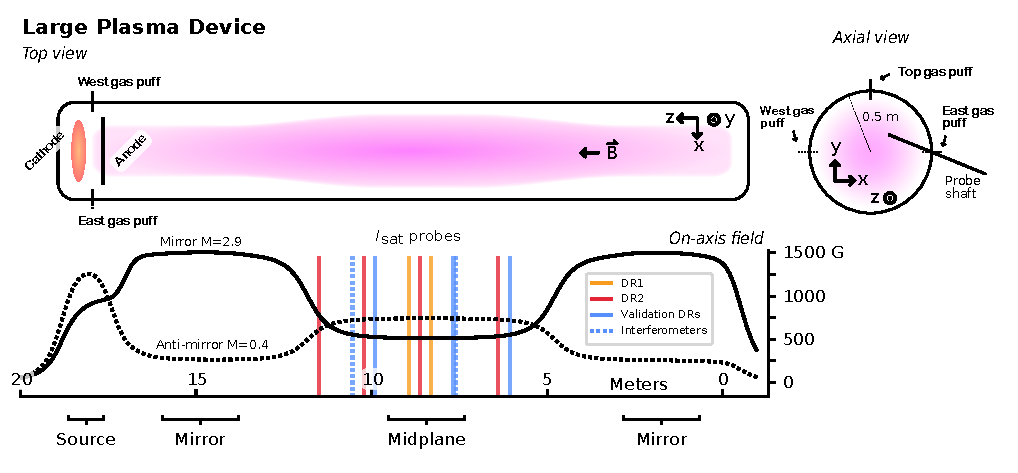
\includegraphics[width=\textwidth]{figures/LAPD+coordinates.pdf}
	\caption[size=12]{\label{fig:LAPD_coords}A cartoon of the Large Plasma Device, the coordinate system used, examples of a mirror and anti-mirror magnetic field configuration, and probe locations used in this study. The source, mirror, and midplane regions are labeled; the three fields were programmed independently.}
\end{figure*}

\section{Processing of $I_\text{sat}$ signals}

The ion saturation current, denoted as $I_\text{sat}$, is obtained by applying a sufficiently negatively bias to a Langmuir probe to ensure the exclusive collection of ions. This collected current is proportional to $S n_e \sqrt{T_e}$, where $n_e$ and $T_e$ are the electron density and temperature, and $S$ is the effective probe collection area. To account for differences in probe tip geometry, the $I_\text{sat}$ values are normalized to area. Under typical conditions, an $I_\text{sat}$ value of 1 mA/mm$^2$ corresponds to $n_e \approx 1\text{-}2\times 10^{12}$ cm$^{-3}$ for a $T_e$ from 4 to 1 eV.

$I_\text{sat}$ measurements were averaged over 10 to 20 ms to exclude plasma ramp-up and fluctuations. Example $I_\text{sat}$ probe data can be seen in fig. \ref{fig:PP1_time-series-example} along side gas puff timings.  For the probe tip that was on the same shaft as the swept probe (in \texttt{DR2}), the signal was instead averaged over when the bias voltage on the swept tip was held constant at the lowest value. A 40 $\mu$s (250 sample) buffer was used after the sweep was turned off to minimize the impact of transient conditions. A comparison of the full trace and the trace with the swept portion excluded can be seen in fig. \ref{fig:PP1_swept_probe}. Notably, the measured $I_\text{sat}$ value does not attain a steady state before the discharge shuts off. 

\begin{figure}
	\centering
	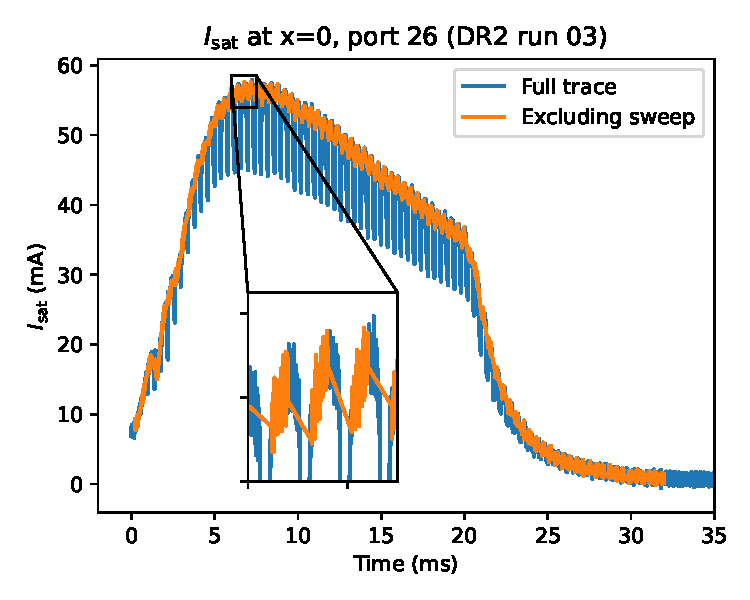
\includegraphics[width=270pt]{figures/PP1_isat_swept_probe.pdf}
	\caption[size=12]{\label{fig:PP1_swept_probe}$I_\text{sat}$ traces from the swept probe (port 26) from \texttt{DR2} datarun 03, shot 1 of 6. The orange curve is excluding times when a sweep is active on an opposing tip. }
\end{figure}

Profile evolution is not studied to minimize computational requirements. $I_\text{sat}$ characteristics vary significantly between axial (z) position machine parameters. For $I_\text{sat}$ measurements on the same probe as a Langmuir sweep (\texttt{DR2} port 26, z=863 cm), the averaging process excludes the sweep period with an additional 40 $\mu$s buffer. $I_\text{sat}$ measurements in \texttt{DR1} that saturated either the isolation amplifier or digitizer are excluded from the dataset. Only 484 shots were removed out of $\approx$132,000, so the impact on the aggregate dataset is minimal. 

\begin{figure}
	\centering
	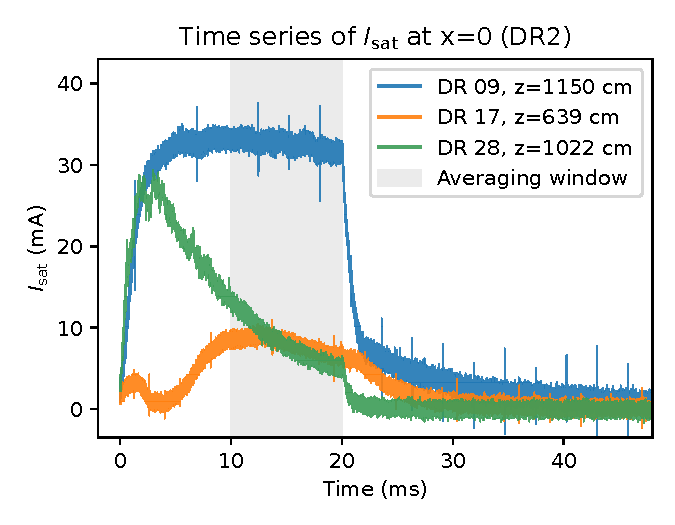
\includegraphics[width=370pt]{figures/PP1_time-series-example.pdf}
	\caption{\label{fig:PP1_time-series-example}Gas puff timings and example $I_\text{sat}$ time series at three different z-axis locations from three different dataruns. Note that some discharges do not achieve steady state in $I_\text{sat}$. }
\end{figure}

While $I_\text{sat}$ exhibits a small degree of shot-to-shot variation, the present model only learns the expected value, leaving distributional modeling to future generative approaches. An example of these $I_\text{sat}$ profiles and the six-shot variance can be seen in fig. \ref{fig:PP1_isat_example}.

\begin{figure}
	\centering
	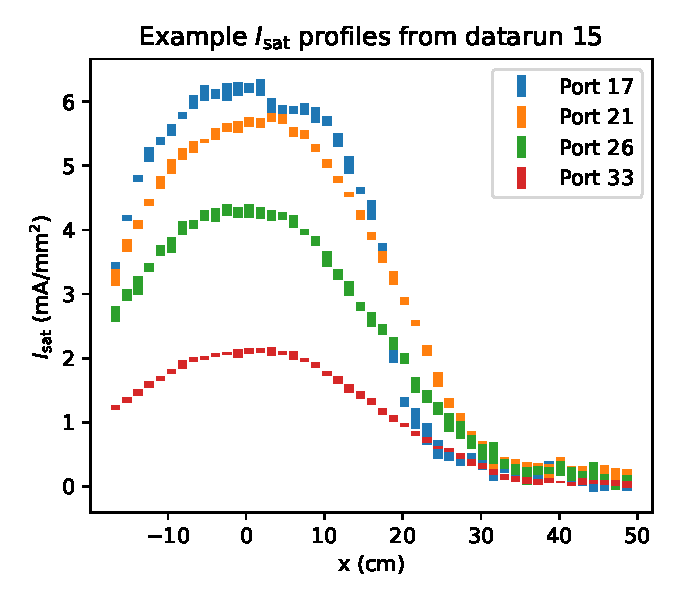
\includegraphics[width=270pt]{figures/PP1_isat_example_bars.pdf}
	\caption[size=12]{\label{fig:PP1_isat_example}Examples of $I_\text{sat}$ profiles from \texttt{DR2} run 15. The bars represent the minimum and maximum of the six $I_\text{sat}$ measurements taken at that position. }
\end{figure}

\section{Model development and training}
\label{sec:model_dev}

\subsection{Model inputs}

Neural network inputs comprise 12 variables: source field, mirror field, midplane field, gas puff voltage, discharge voltage, gas puff duration, probe coordinates (x, y, z), probe rotation, run set identifier, and top gas puff flag. These variables can be interpreted as six control parameters, four probe coordinates, and two flags. These inputs are mean-centered and normalized to the peak-to-peak value with no outliers in the dataset. The baseline models trained in section \ref{sec:baselines} did not contain the run set identifier or top gas puff flag.

\subsection{Training details}

For initial experiments in training the model, a mean-squared error (MSE) loss is used:
\begin{equation}
	\mathcal{L}_\text{MSE}=\frac{1}{m}\sum_{i=1}^m \left(f\left(x_i\right) - y_i \right)^2
\end{equation} 
where $x_i$ represents the input vector for the $i$th example, $y_i$ the target measurement, $m$ the batch size, and $f$ the NN. During training, overfitting was assessed via the validation set MSE with a traditional 80-20 train-validation random split. Unless stated otherwise, a dense neural network, 4 hidden layers deep and 256 units wide (201,218 parameters for $\beta$-NLL loss, 200,962 parameters for MSE loss), was trained with AdamW using a learning rate of $3\times10^{-4}$. Leaky ReLU activations (the nonlinearities in the NN) and adaptive gradient clipping\cite{seetharaman_autoclip_2020} (cutting gradients norms above the 90th percentile of recent norms) were used to mitigate vanishing gradients and mitigate exploding gradients, respectively. The models were evaluated after training concluded at 500 epochs.

\subsection{Validating the training pipeline}

ML training processes are relatively simple but bugs, particularly in the data pipeline, can be insidious and can affect final model performance even though training looks fine. Here we validate the data pipeline (which should be performed in every ML study) to verify that the model is training and expected and that there is no accidental data leakage between the train and test sets. Andrej Karpathy's advice for training neural networks \cite{karpathy_recipe_2019} was used as a template for verifying the training procedure used in this project. The data fed into the model immediately before the forward pass (and subsequent backpropagation) was stored and verified: the data are correctly randomly shuffled in each batch. Each epoch contains the same random shot order. To validate the data pipeline, a simple dense model (4 layers, 512 wide with one output; 794113 parameters, tanh activations) was trained. The model is also overfit on a single batch (128 examples) of training data to make sure that training progresses as expected. A deep double descent is observed as expected \cite{nakkiran_deep_2019,schaeffer_double_2023}. Training on a batch of 8 examples reaches $\approx$ 0 training loss after 50 steps. Plots of the train and validation losses can be seen in Fig. \ref{fig:PP1_overfit_losses}.

Multiple models were trained with varying depths and widths to verify that training loss decreases with increased model capacity. Doubling the layer width from 512 to 1024 moderately decreases the training loss; doubling the depth of the network from 4 to 8 layers has a larger impact. Increasing the width further to 2048 and depth to 12 layers has a dramatic impact on training loss, so this model and dataset are behaving nominally. The model pipeline is training and performing as expected, so we proceed.

\begin{figure}
	\centering
	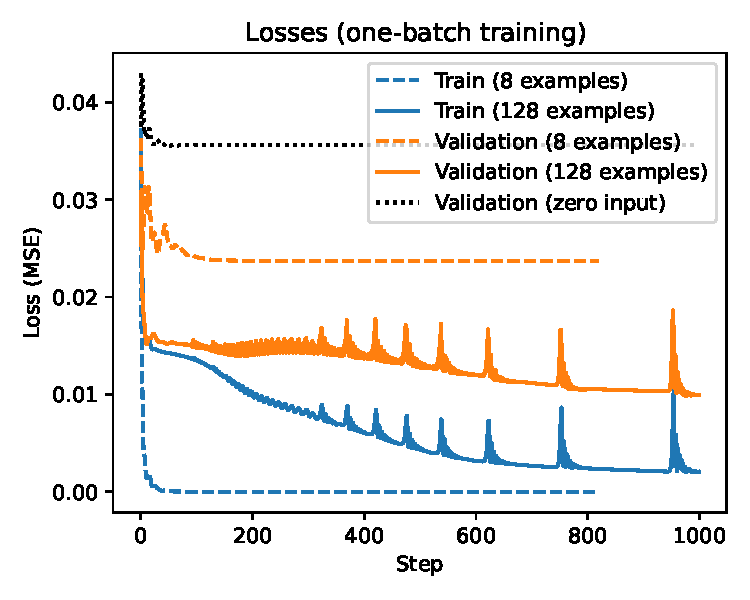
\includegraphics[width=300pt]{figures/PP1_overfit_losses.pdf}
	\caption[size=12]{\label{fig:PP1_overfit_losses}Training and validation losses when overfitting the model. A deep double descent in the validation losses is observed when fitting a single batch of 128 examples. The 8-example batch hits near-zero loss after 50 steps. This process verifies our training process is functioning as expected. The spikes are from exploding gradients which can be mitigated by clipping the gradients. A model trained on blank data is also shown as the black dotted line.}
\end{figure}

\subsection{Baselines for mean-squared error}
\label{sec:baselines}

A model was first trained with zeroed-out inputs as a baseline and to validate the data pipeline. This model effectively has only a single, learnable bias parameter at the input. This process yields a validation loss (simply MSE in this case) of 0.036. 

%A linear model, though incapable of reasonably fitting the data, was trained as a performance baseline and to validate the data pipeline. This baseline linear model reaches a training and validation loss (MSE) of around 0.014. These initial models used \texttt{tanh} activations, though the impact of using a different activation function is minimal in these cases.
%\subsubsection{Baseline linear-like models (\texttt{DR2})}
A linear model obviously cannot fit the dataset (see the nonlinear shape of the profiles in fig. \ref{fig:PP1_isat_example}). However, a simple (and mostly linear) model can provide a performance baseline to help spot bugs when training more complex models. Since the x- and y- profiles have a approximate $\tanh$ shape, a feature is added at the linear model input stage for the x and y coordinates: $x_\texttt{tanh} = c \cdot \tanh\left(\left|x + s\right| \cdot a + b \right)$ where $s, a, b, c$ are trainable parameters (independent for each coordinate; $c$ is superfluous). This function was chosen to give the linear model the capability of expressing $\tanh$-like curves. The performance of the linear model on \texttt{DR2} data, with and without the $\tanh$ features, can be seen in fig. \ref{fig:PP1_linear_simple_data}. This baseline linear-like model reaches a training and validation loss of around 0.011, with the RMSE $=\sqrt{\text{loss}} \sim 0.1$. The linear-only model is marginally worse with losses at around 0.014.

\begin{figure}
	\centering
	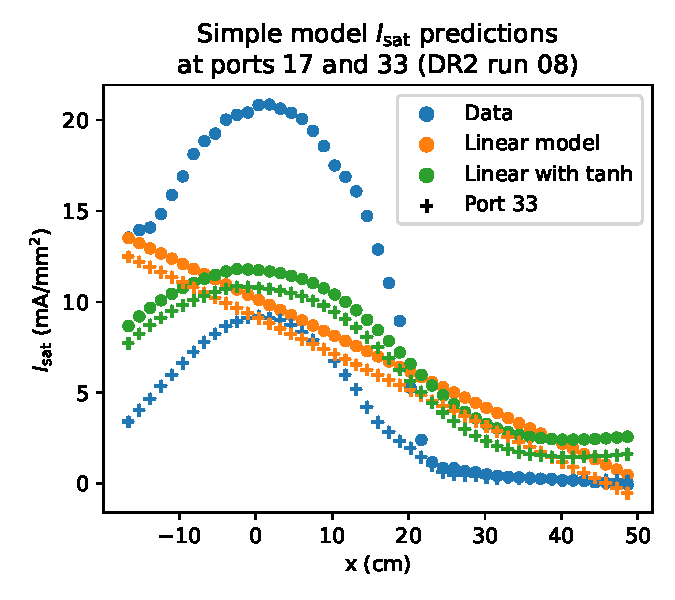
\includegraphics[width=300pt]{figures/PP1_linear_simple_vs_data.pdf}
	\caption[size=12]{\label{fig:PP1_linear_simple_data}$I_\text{sat}$ profiles and predictions for ports 17 and 33 based on inputs from \texttt{DR2} run 08 using a liner and linear-with-tanh models. \texttt{DR2} run 08 is in the training set. The ``data'' points are averaged over six shots. Run 08 was chosen for its representative performance; ports 17 and 33 were chosen to demonstrate the maximal axial variation (across 511 cm). These models fail to describe the data accurately.}
\end{figure}

This feature engineering-like approach can continue. For example, the width of the profile is largely controlled by magnetic field configuration of the device, particularly by $\sqrt{B_\text{midplane}/B_\text{source}}$. This behavior can be added to this model, either as a new feature or as a custom relationship in the model. Note that, as seen in fig. \ref{fig:PP1_linear_simple_data}, the width of the profile also depends on the axial coordinate. Combined with other coordinates and actuators, like discharge voltage and gas pressure, the number of possible features or function space grows combinatorially, making this custom fitting process difficult and tedious to design and test by hand. The obvious solution would be to use symbolic regression or fitting to a function library which may be  ideal methods if simple profile prediction were the final goal. However, we are ultimately interested inferring trends in a much more complex input space where neural networks are more flexible and accurate. If NNs do face generalization issues, symbolic regression or a SINDy-like approach can used instead, albeit with limited applications. Symbolic methods are appealing because the fits are simple. However, even though a simple equation may fit the data well, it does not necessarily provide insight or relate to the underlying physics; using a freeform fitting function like a neural network is more appropriate in this use case.

A summary of these baselines is seen at the top of Table \ref{tab:loss_summary}.


\begin{table}
	\small
	\centering
	\caption{Summary of test set losses for different training data and ensembles}
	\label{tab:loss_summary}
	\begin{tabular}{l l l}
		Model & MSE $\times 10^{-3}$ \\
		\hline
		Zeroed-input & 36  (validation) \\
		Linear model & 14 (validation) \\
		Linear with tanh features & 11 (validation)\\
		\hline
		9 dataruns & 7.0\\
		19 dataruns & 6.9 \\
		29 dataruns & 4.2 \\
		39 dataruns & 4.1 \\ 
		49 dataruns & 3.4 \\
		\texttt{DR1} only & $6.4$ \\
		\texttt{DR2} only & $5.4$ \\
		Full set, large model & $2.8$ \\
		Full set average & $3.6 \pm 0.56$ \\
		Full set ensemble & $2.9 \pm 1.1$ \\
		\hline
		``Run set'' flag average & $2.1 \pm 0.15$ \\
		``Run set'' flag ensemble & $1.9 \pm 0.64$ \\
		``Top gas puff'' flag & 1.8 \\
		
	\end{tabular}
\end{table}

\subsection{Effects of training set and model sizes}
 
To study the effects of reduced diversity, the number of unique dataruns in the training set was systematically reduced while evaluating on a fixed test set. The test set loss monotonically increased with this decrease in datarun count. Part of this decrease may be caused by a simple reduction in training set size. In addition, models were individually trained and evaluated on \texttt{DR1} only or  \texttt{DR2} only. When evaluated on the left-out run set, the test set losses were high, near or above the zero-input baseline of $3.6 \times 10^{-2}$. This result suggests that both run sets contain significant information missing in the other, and training on both provides beneficial information on the structure of the $I_\text{sat}$ measurement despite different probe calibrations and cathode state.

A larger model, consisting of a 12-deep 2048-wide dense network, was trained on the full training dataset, evaluated at 30 epochs. This larger model yielded a test MSE of $2.8 \times 10^{-3}$, indicating that these NNs are behaving as expected. Longer training or larger models may yield better test set results, but will likely not come close to the training and validation losses which are on the order of $10^{-5}$. Combined models with differing initializations (an ensemble), were trained to measure the MSE variance over model parameters which was about 16\%. When the $I_\text{sat}$ predictions were averaged, the test set MSE was $2.9 \pm 1.1 \times 10^{-3}$, achieving the best performance for that model size. These test set losses are also seen in Table \ref{tab:loss_summary}. 

%One unexpected result is that models trained on a single run set appear to perform worse when evaluated on the test set (from that particular run set) compared to the mixed training set of the same size (green arrows vs blue x). This fact indicates that mixing dataruns, despite different probe calibrations and cathode state, provides beneficial information on the structure of the $I_\text{sat}$ measurement. This model is able to leverage information in both dataruns despite potential differences in the effect of the machine settings and the cathode condition.

%Skepticism is warranted, however, because the variance over model parameters may be able to account for most, if not all, of the performance difference as suggested by the full-set ensemble. The variance caused by random datarun selection may also account for some of the difference; this variance was not measured and could be considerable. The effect of varying the training and test datasets will be discussed in section \ref{subsec:cross-validation}.

\subsection{Improving performance with machine state flags}

Data from \texttt{DR1} and \texttt{DR2} were collected 14 months apart leading to differing machine states. In \texttt{DR1}, only one turbo pump was operating leading to much higher neutral pressures than in the \texttt{DR2} run set. A new parameter (mean-centered and scaled) was added to the inputs to distinguish between these two run sets. All the predictions in this study use the \texttt{DR2} run set flag (a value of 1.0) because turning off the turbopumps is not a commonly desired mode of operating the LAPD. The inclusion of this parameter also provides the model the ability to distinguish between the probe calibration differences between \texttt{DR1} and \texttt{DR2}. An ensemble prediction with this run set flag brings the test set MSE down to $1.9 \times 10^{-3}$.  

A flag indicating when the top gas puff valve was enabled in \texttt{DR2} was also added to all training data, allowing the model to further distinguish between different fueling cases. The addition of this flag incrementally improved test set MSE to $1.8 \times 10^{-3}$. The effect on MSE on the inclusion of these new parameters is compared to the performance of other models in Table \ref{tab:loss_summary}. 

\subsection{Learning rate scheduling}
Modifying the learning rate over time (scheduling) is known to improve model learning. The following schedules were compared: constant learning rate ($\gamma = 3 \times 10^{-4}$), $\gamma \propto \text{epoch}^{-1}$, $\gamma \propto \exp{(-\text{epoch})}$, and $\gamma \propto \text{epoch}^{-1/2}$. The epoch is the training step divided by the number of batches in one epoch, so ``epoch'' in this case takes on a floating-point value. $\gamma \propto \text{epoch}^{-1}$ appears to give the best test set loss by a test MSE difference of $1 \times 10^{-4}$, and any schedule beats a constant learning rate by a difference of $2-4 \times 10^{-4}$. 
%The differences in test set losses are small, but the difference in training and validation losses are quite significant, with the constant learning rate loss being three times higher. 

%\begin{enumerate}
%	\item Baseline models plot (done)
%	\item Losses vs dataset diversity (done)
%\end{enumerate}
 
%\begin{figure}
%	\centering
%	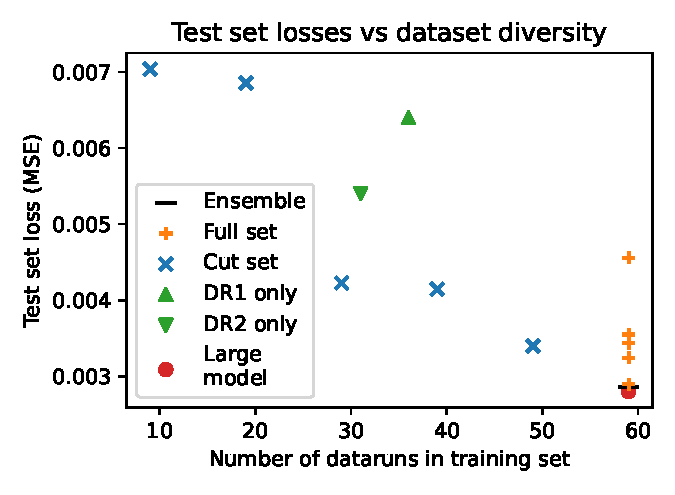
\includegraphics[width=\columnwidth]{figures/PP1_test-loss_vs_dataset.pdf}
%	\caption[size=12]{\label{fig:PP1_validation_diversity}Several models were trained with dataruns cut out, decreasing the diversity of the training set. The test set was kept fixed. Loss on the test set monotonically increases with decreasing diversity. }
%\end{figure} 

\section{Uncertainty quantification}
\label{sec:uncertainty}

\subsection{$\beta$-NLL loss}

Instead of predicting a single point, the model can predict a mean $\mu$ and variance $\sigma^2$ using the negative-log likelihood (NLL) loss \cite{nix_estimating_1994,lakshminarayanan_simple_2017} by assuming a Gaussian likelihood. An adaptive scaling factor $\text{StopGrad}(\sigma_i^{2\beta})$ is introduced that can be interpreted as an interpolation between an MSE loss and Gaussian NLL loss, yielding the $\beta$-NLL loss:

\begin{equation}
%	\begin{multline}	
	\mathcal{L}_{\beta-\text{NLL}} = \frac{1}{2}\left( \log{\sigma^2_i(\mathbf{x}_n)} +\frac{\left(\mu_i(\mathbf{x}_n) - y_n\right)^2}{\sigma^2_i (\mathbf{x}_n)} \right) \text{StopGrad}\left(\sigma_i^{2\beta}\right)
	\label{eq:loss_beta-NLL}
%	\end{multline}
\end{equation}

for example $n$ and model $i$, with an implicit expectation over training examples. $\beta=0$ yields the original Gaussian NLL loss function and $\beta=1$ yields the MSE loss function. This factor improves MSE performance by scaling via an effective learning rate for each example (which necessitates the \texttt{StopGrad} operation) \cite{seitzer_pitfalls_2022}, and improves both aleatoric and epistemic uncertainty quantification \cite{valdenegro-toro_deeper_2022}. $\beta=0.5$ was used by default in this study. This $\beta$-NLL loss function also improved training stability.

This NLL-like loss assumes the prediction -- the likelihood of $y$ given input $\mathbf{x}$: $p(y|\mathbf{x})$ -- follows a Gaussian distribution. Treating each prediction as an independent random variable (considering each model in the ensemble is sampled from some weight distribution $\theta \sim p(\theta | \mathbf{x}, y)$) and finding the mean of the random variables yields a normal distribution with mean $\mu_* (\mathbf{x}) = \langle \mu_i(\mathbf{x}) \rangle $ and variance $\sigma^2_* = \langle \sigma^2_i(\mathbf{x}) + \mu^2_i(\mathbf{x}) \rangle - \mu^2_* (\mathbf{x})$ where $\langle \rangle$ indicates an average over the ensemble.

The loss function for one of the NNs in an ensemble is seen in fig. \ref{fig:beta-NLL_loss-mse}. The MSE decreases monotonically for the training and validation set, but does not for the test set. The loss function can no longer be interpreted as a log-likelihood because of the effective per-example learning rate set by the $\beta$ term in the loss (eq. \ref{eq:loss_beta-NLL}). Note that early stopping (at around 8 epochs) would improve the test set loss, but the MSE would still be several factors higher than after 500 epochs. Early stopping was not explored in this study.

\begin{figure}
	\centering
	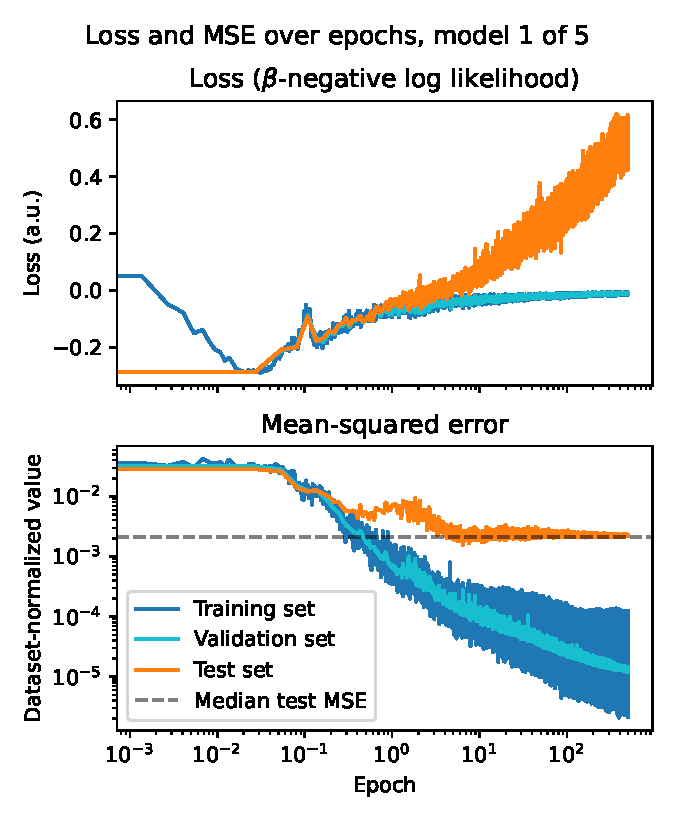
\includegraphics[width=300pt]{figures/beta-NLL_loss-mse.pdf}
	\caption[size=12]{\label{fig:beta-NLL_loss-mse}The loss and MSE for the training, validation, and test sets over the entire training duration of 500 epochs. The inclusion of the $\beta$ term in the loss function -- interpreted as a per-example learning rate -- makes the loss function no longer interpretable in simple terms. The mean-squared error benefits from longer training for all sets.}
\end{figure}

The ensemble predictive uncertainty can be broken down into the aleatoric and epistemic components \cite{valdenegro-toro_deeper_2022}: the aleatoric uncertainty is $\langle \sigma^2_i (\mathbf{x}) \rangle$ and the epistemic uncertainty is $\langle \mu^2_i (\mathbf{x}) \rangle - \mu^2_* (\mathbf{x}) = \text{Var}\lbrack\mu_i (\mathbf{x}) \rbrack$. The intuition behind these uncertainties is that the random fluctuations in the recorded data are captured in the variance of a single network, $\sigma^2_i$. If the choice of model parameters were significant, we would expect the predicted mean for a single model, $\mu_i$, to fluctuate as captured by $\text{Var}\lbrack\mu_i (\mathbf{x}) \rbrack$. 

%Using the $\beta$-NLL loss, the model is slightly better calibrated, but barely worth discussing. 

%\begin{enumerate}
%	\item Cross validation plot (done)
%	\item z-score histogram (done)
%	\item Calibration via weight decay scan (done)
%	\item Profiles with different weight decays (done)
%\end{enumerate}

\subsection{Cross-validation MSE}

For cross-validation, multiple train-test set pairs were created. Test set 0 comprises deliberately chosen dataruns to encompass a diverse set of machine settings and probe movements. The other six datasets were  compiled with randomly chosen dataruns (without replacement) while keeping the number of dataruns from \texttt{DR1} and \texttt{DR2} equal. Seven model ensembles (5 NNs per ensemble -- 35 NNs total) were trained to evaluate the effect of test set choice on model MSE. The test set MSE performance can be seen in fig. \ref{fig:cv-beta-NLL-test-mse}, and the training MSE performance in fig. \ref{fig:cv-beta-NLL-train-mse}. The median ensemble test set MSE for these seven sets was $2.13 \times 10^{-3}$ with a mean of $3.6 \times 10^{-3}$. The handpicked dataset had an ensemble test set MSE of $1.85 \times 10^{-3}$, indicating that the choice of dataruns was adequately representative. This median MSE will be used to estimate model prediction error in addition to uncertainty quantification. This cross-validation also provides an error estimate if the models were to be trained on \emph{all} dataruns. Ensembles always out-performed the average error of single-model predictions.

All validation set MSEs fall between $1$ and $6 \times 10^{-5}$, with the average training MSE falling within that range as well. These MSEs indicate that the model is able to fit the training data to a high degree of accuracy regardless of which dataruns are held out. The loss and MSE curves over training epochs can be seen in the appendix in fig. \ref{fig:beta-NLL_loss-mse}.

%The median of the cross-validation ensemble performance for the test set is roughly the same as the MSE for testing set 0, so our choice of dataruns for the testing set appears reasonable. The calibration of the model also varies across dataruns, which can be investigated. Ideally, knowing the models train well and having an idea of the cross-validated error, it should be possible to train on all data in it's entirety and still have some reasonable estimate of the error of the model.

\begin{figure}
	\centering
	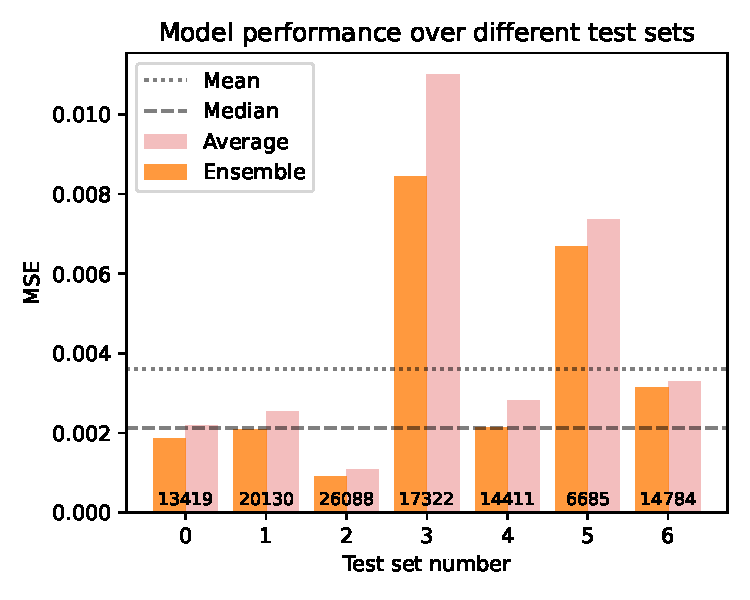
\includegraphics[width=260pt]{figures/cv-beta-NLL-valid-mse.pdf}
	\caption[Cross-validation test set error]{\label{fig:cv-beta-NLL-test-mse}Model performance as measured by MSE over test sets with different dataruns. Test set 0 is the hand-picked dataset, and the rest were randomly compiled without replacement (though separate for \texttt{DR1} and \texttt{DR2}). The number at the bottom of the bar chart is the number of shots in the testing set. The median test set performance is very close to the hand picked (set 0) performance. Ensembles always out-perform the average single-model prediction.}
\end{figure}

\begin{figure}
	\centering
	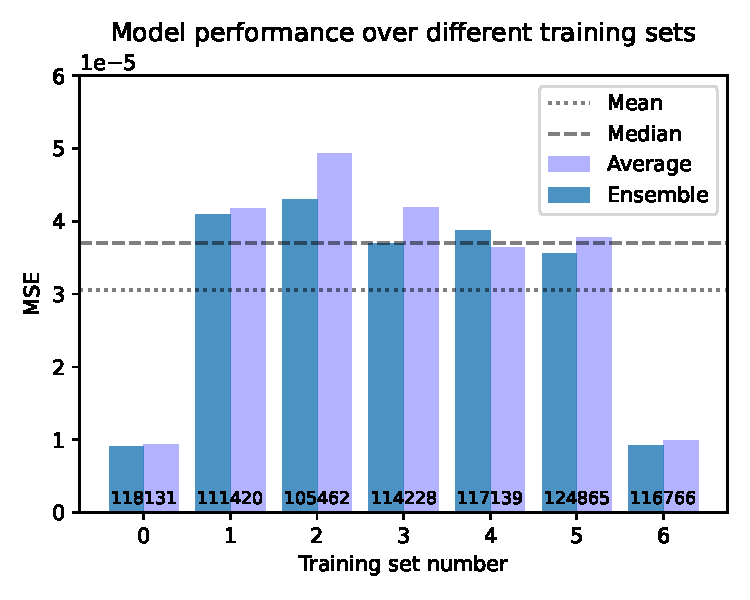
\includegraphics[width=260pt]{figures/cv-beta-NLL-train-mse.pdf}
	\caption[Cross-validation training set error]{\label{fig:cv-beta-NLL-train-mse}See caption for fig. \ref{fig:cv-beta-NLL-test-mse}. Note that the training loss is dramatically less than the testing loss, but otherwise there is no discernible trend.}
\end{figure}

\subsection{Model calibration via weight decay}

The predicted uncertainty may not provide an accurate range of $I_\text{sat}$ values when compared to the measured value. Calibrating the model means changing the predicted uncertainty range so that the measured values fall within that range according to some distribution, such as a Gaussian in this case. One of the ways assessing this calibration is by the z-score of predictions, where $z_n= \left(x_n - \mu_n \right) / \sigma_n(x_n)$ for example $x_n$, predicted mean $\mu_n$, and standard deviation $\sigma_n$. Perfect model calibration would lead to identical z-score distribution $\mathcal{N}(\mu=0, \sigma=1)$ for the training a test sets. When evaluated on the training set, the distribution should be a Gaussian with a standard deviation of 1. The z-score disbitrubtions for the train and test sets with a model weight decay of 0 can be seen in fig. \ref{fig:z-score_wd-0_paperplot}.

\begin{figure}
	\centering
	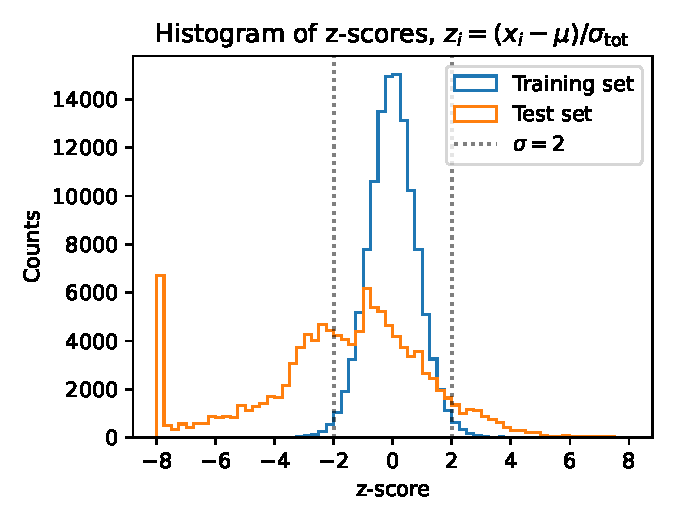
\includegraphics[width=300pt]{figures/z-score_wd-0_paperplot.pdf}
	\caption[Z-score distributions for the training and test sets for $\lambda = 0$]{\label{fig:z-score_wd-0_paperplot}Z-scores for the training and testing set for the model with a weight decay coefficient $\lambda$ of zero. The magnitude of counts for the test set is scaled up by a factor of 8.8 (the train-to-test example ratio). The histograms are clipped between z of -8 and 8 with a bin width of 0.25; the spike at the negative side of the test set histogram is from the long tail.}
\end{figure}

Increased weight decay can lead to better model calibration \cite{guo_calibration_2017}. Weight decay penalizes large parameter values by adding the L2 norm of model weights to the loss. Model ensembles were trained with weight decay coefficients between 0 and 50 to determine the best calibrated model determined by the distribution of z-scores of the training and test sets. The results of this weight decay scan are seen in Fig. \ref{fig:beta-NLL_wd_model_performance}. Increasing the weight decay increases the test MSE and decreases its z-score standard deviation. This large standard deviation is caused by outliers. Excluding z-scores magnitudes above 10, or 4.4\% of the test set, yields a standard deviation of 2.53. This long tail indicates that the distribution of predictions on the test set is not Gaussian. Nonetheless, the trend remains that increasing weight decay leads to smaller test set z-score standard deviations. However, the test set MSE increases after a weight decay of 1. This increase in test MSE implies that the model is making less accurate predictions but is better calibrated. Highly biased models are better calibrated, but come at great expense of mean prediction error. At the weight decay value of 50, the model has worse error than a linear model. Despite the attempts using weight decay, the model never becomes well-calibrated: the predicted uncertainty is always too low by a factor of 2 to 5. 

%As seen in Fig. \ref{fig:extrapolation-variance_wd-comparison}, the uncertainty predictions are not useful except for models with low weight decays.
 
%A comparison of many different weight decay coefficients can be seen in Fig. \ref{fig:weight_decay-model}; 20 was determined to be a good weight decay value. The ``knee'' value of 30 was not chosen because the distribution of z-scores looked odd. The training and test z-score distribution can be seen in Fig. \ref{fig:weight_decay-distribution}. Note that weight decay (coefficient $\lambda$) is implemented in \texttt{AdamW} as $\theta_t = \theta_{t-1} -\gamma\lambda \ \theta_{t-1}$ so learning would be impossible above the reciprocal of the learning rate of $\gamma = 3 \times 10^{-4}$.

%Despite a well-calibrated test set error, the predictions on the training and test sets are not very good. An MSE of $\approx 3 \times 10^{-3}$ may sound decent (RMSE of $\approx 5\%$) but the error is weighted by the low $I_\text{sat}$ values at the edge of the plasma (see Fig. \ref{fig:PP1_02_isat_distribution}) which are relatively easy to predict correctly. 

\begin{figure}
	\centering
	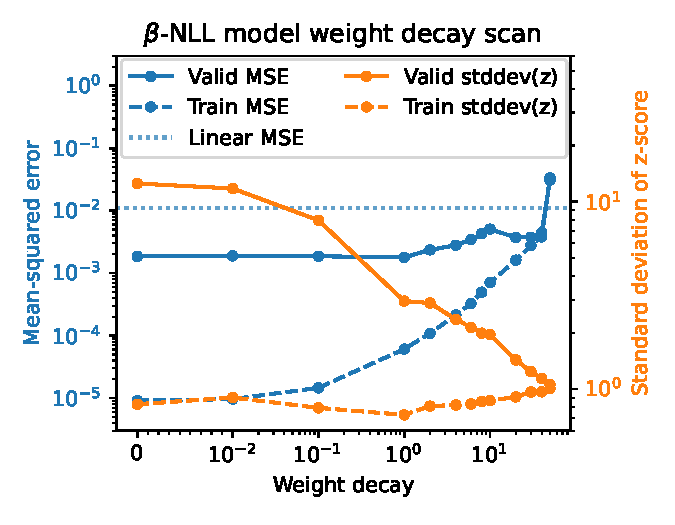
\includegraphics[width=300pt]{figures/beta-NLL_wd_model_performance.pdf}
	\caption[size=12]{\label{fig:beta-NLL_wd_model_performance}Model performance and calibration for different weight decays. Highly biased models are better calibrated, but come at great expense of mean prediction error. At the weight decay value of 50, the model has worse error than a linear model. Note the linear scale below $10^{-2}$.}
\end{figure}

Despite the better calibration, the uncertainty predicted by a model with a large weight decay is decidedly worse: the uncertainty is similar across an entire profile, and when projected beyond the training data, the total uncertainty remains largely constant as seen in Fig. \ref{fig:extrapolation-profile-var_two}. The zero weight decay model exhibits relatively increasing uncertainty beyond the bounds of the training data. Although not well-calibrated, this uncertainty can provide a hint of where the model lacks confidence relative to other predictions, even though the uncertainty is much less than it should be.

\begin{figure*}
	\centering
	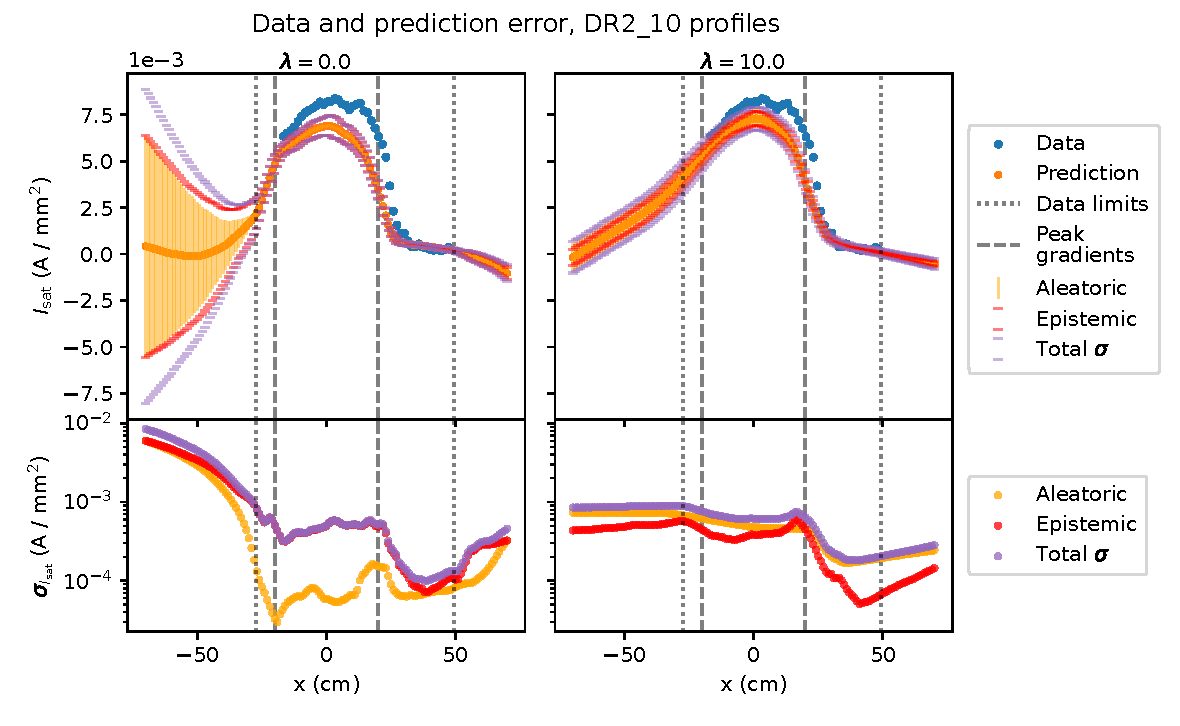
\includegraphics[width=\linewidth]{figures/extrapolation-profile-variance_DR2_10_wd-comparison_two.pdf}
	\caption[size=12]{\label{fig:extrapolation-profile-var_two}Model extrapolation performance (top plots) with uncertainty (bottom plots) for a model ensemble trained on a $\beta$-NLL loss function. \texttt{DR2} run 10 was chosen as an illustrative example. The \em relative \em uncertainty appears to be more useful when zero weight decay ($\lambda = 0$, left) is used: the uncertainty increases when the model is predicting outside its training data along the x-axis.}
\end{figure*}

\section{Evaluating model performance}
\label{sec:validation}

Model performance is evaluated in three ways by comparing against intuition from geometry, an absolute measurement, and extrapolated machine conditions. 

%\begin{enumerate}
%	\item Geometrical changes with changing mirrors (done)
%	\item Single shot prediction (done)
%	\item Extrapolation plot comparison (done)
%\end{enumerate}

\subsection{Checking geometrical intuition}

Assuming magnetic flux conservation, we know that modifying the mirror geometry can control the effective width of the plasma. One way to check that the model is learning appropriate trends is to check with this intuition. If the magnetic field at the source is not equal to the field at the probe, the probe will see the plasma expanded (or contracted) by roughly a factor of $\sqrt{B_\text{probe}/B_{source}}$. The cathode is about 35 cm in diameter, so a magnetic field ratio of 3 would give produce a plasma approximately 60 cm in diameter. All the probes used in this study are in or very close to the zero-curvature midplane region of a mirror.

To check this intuition, the model is given the following inputs: $B_\text{source}$=500 G, $B_\text{mirror}$=1500 G, $B_\text{midplane}$=500 G, discharge voltage=110 V, gas puff voltage=70 V, gas puff duration=38 ms, run set flag=\texttt{DR2} and top gas puff=off. The discharge voltage and gas puffing parameters were arbitrarily chosen. The x coordinate is scanned from 0 to 30 cm, and the z coordinate from 640 to 1140 cm. This discharge is then modified by separately changing $B_\text{source}$ to 1500 G and $B_\text{midplane}$ to 750 G (M=1.5). %and $B_\text{mirror}$ to 750 G. 
The x profiles at the midplane (z=790 cm) of the reference M=3 prediction, source field change, and midplane field change, all scaled to cathode radius, can be seen in Fig. \ref{fig:changing-B-field_M=3_x-prof}. Changing the source field to 1500 G increases the $I_\text{sat}$ towards the edge of the plasma, as expected. When the midplane field is increased, the $I_\text{sat}$ values decrease at the edge and increase at the core (x=0 cm), implying a thinner plasma column and is consistent with previously measured behavior. When only the mirror field is modified (not shown), the strongest effect on $I_\text{sat}$ is on or near x=0 cm, and the plasma column width does not appear to appreciably change. 
%Strong axial $I_\text{sat}$ gradients are present in these predicted discharges.

\begin{figure}
	\centering
	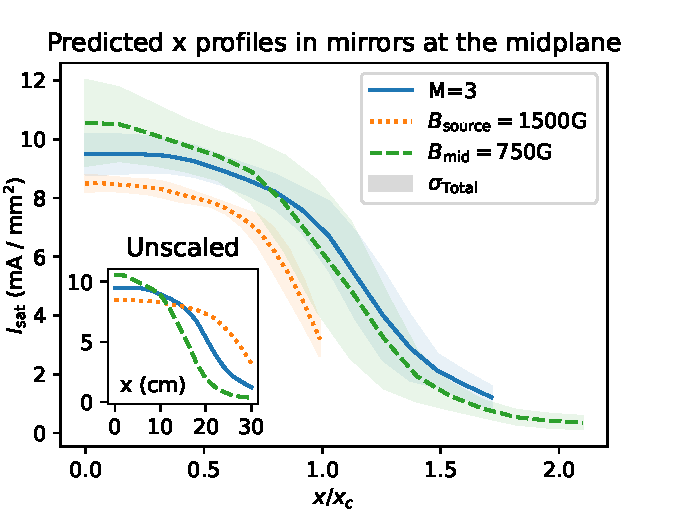
\includegraphics[width=300pt]{figures/changing-B-field_M=3_x-prof.pdf}
	\caption[size=12]{\label{fig:changing-B-field_M=3_x-prof}Plot of various mirror configurations scaled to the cathode radius $x_c=17.5$ cm at the midplane (z=790 cm). When scaled according to the expected magnetic expansion, the profiles generally agree. The smaller the plasma diameter (and thus smaller volume), the higher the peak in $I_\text{sat}$ at the core, as expected. }
\end{figure}

\subsection{Directly comparing prediction to measurement}

%Data were collected on September 18th, 2024 to validate the predictions made for the strongest axial variation. Given the model inputs were incorrect (the gas puff voltage was swapped with discharge voltage), this optimization is broadly wrong. However, because the prescribed gas puff voltage and discharge voltage were the same (90 V) and within the bounds of the actuator training data, we can still use these data for validation. 

$I_\text{sat}$ measurements were taken with the following LAPD machine settings: $B_\text{source}$=1250 G, $B_\text{mirror}$=500 G, $B_\text{midplane}$=1500 G, discharge voltage=90 V, gas puff voltage=90 V, gas puff duration=38 ms, run set flag=\texttt{DR2} and top gas puff=off. These settings were from a previous discharge optimization attempt. The probes utilized were the permanently-mounted 45$^\circ$ probe drives. These probes were known to have identical effective areas relative to each other from the previous experiment and from analyzing the discharge rampup.

Because of data acquisition issues, only a single useful shot was collected at a nominal -45$^\circ$ angle (relative to the x-axis) 10 cm past the center (x=0 cm, y=0 cm) of the plasma on three probes at z-positions of 990, 767, and 607 cm (ports 22, 29, and 34, respectively). The probe drives were slightly uncentered, leading to the real coordinates of the probes to be around x $=9.75$ cm and y $=-8.4$ cm. Note that the model can predict anywhere in LAPD bounded by the training data, so off-axis measurements are not an issue.
%These probes were also not centered so the positions were slightly further +x and -y. Issues (scripts crashing) with the probe drives and oscilloscope readout resulted in only a single shot being recorded. 
The resulting predictions using these coordinates and machine conditions can be seen in Fig. \ref{fig:measured-vs-predicted}. 
%The off-axis predictions and $I_\text{sat}$ measurements result in less-smooth profile when compared with the on-axis prediction. 
The model reproduces the axial trend well, but slightly underestimates $I_\text{sat}$ on an absolute basis. However, given the lack of absolute $I_\text{sat}$ calibration and variable machine state, the agreement of the absolute $I_\text{sat}$ values may be coincidental. Nevertheless, the trend exhibited by this validation study match the predicted trend and increase our trust in model predictions. 
%\todo{Rephrase to emphasize that we can still trust the model despite calibration differences}

\begin{figure}
	\centering
	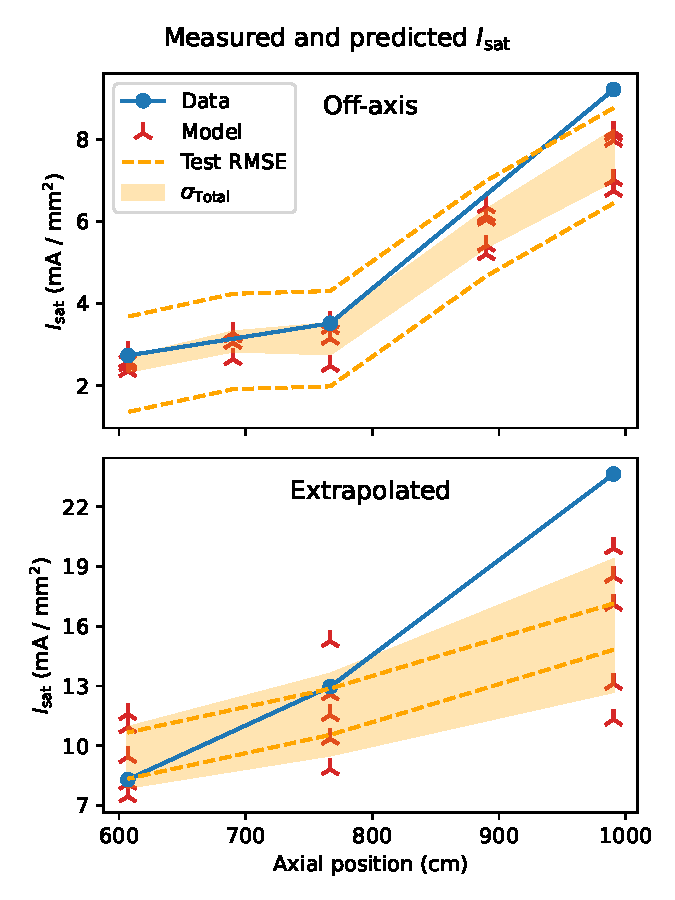
\includegraphics[width=300pt]{figures/measured-vs-predicted_off-axis_160V}
	\caption[size=12]{\label{fig:measured-vs-predicted}Top: data collected at off-axis positions around x $=9.75$ cm and y $=-8.4$ cm are compared with predictions from the machine learning model at the same points in addition to two interpolating predictions. The model predicts the trend well, but underestimates $I_\text{sat}$ in general. The shaded orange region is the total model uncertainty ($\sigma = \sqrt{\text{Var}}$). Bottom: Measured vs predicted $I_\text{sat}$ values for an odd machine configuration with $B_\text{source}$=822 G and discharge voltage=160 V. The training data only covers discharge voltages up to 150 V The machine was also in an odd discharge state, so it's no surprise that the predicted uncertainty bounds are very large (even greater than the test set RMSE value) and that accuracy suffers.}
\end{figure}

An additional validation datarun was performed. For this run, the discharge voltage was increased to 160 V, and the source field changed to 822 G. The training data contains discharge voltages up to 150 V, so this case tests the extrapolation capabilities of the model. The comparison of model predictions and the measured data can be seen in Fig. \ref{fig:measured-vs-predicted}. As stated earlier, the absolute uncertainty provided of the model is not calibrated. However, note that the level of uncertainty provided by the model, as well as the large spread in model predictions, are much greater than seen in the interpolation regime (Fig. \ref{fig:measured-vs-predicted}) and eclipses the cross-validated test set root mean squared error (RMSE). We conclude that this model has good interpolation capabilities, but extrapolation -- as with any model -- remains difficult.

%Probe tip rotation was not accounted for in the prediction, but including the correct rotation produces uncertainty meeting or exceeding the test RMSE threshold because rotations at this angle have not been seen by the model. This probe tip rotation bias suggests that for this model probe rotation need not be correct for accurate predictions. The model performs worse when azimuthal symmetry is assumed by treating x as the radial coordinate and calculating the distance from x=y=0 cm. This degraded inference performance, also seen when training the model (section \ref{subsec:azimuthal_symmetry}) suggests that there is some intrinsic azimuthal asymmetry in the plasma, possibly caused by the horizontal gas puff injection near the source.

\subsection{Comparison with Thomson scattering}

The z-axis interpolation for dataruns in the training and test sets can be evaluated using the Thomson scattering (TS) diagnostic. The TS measurement is taken 8 ms into the discharge for \texttt{DR1} 12 ms into the discharge for \texttt{DR2}, but in this study the measured and predicted $I_\text{sat}$ are instead averaged over 10 to 20 ms. The Thomson scattering measurement is compared in with \texttt{DR1} and \texttt{DR2} in figs. \ref{fig:DR1_vs_TS} and \ref{fig:DR2_vs_TS}, respectively. The linear slope fits do not take model error into account In \texttt{DR1}, $I_\text{sat}$ predictions disagree with the $I_\text{sat}$ derived from TS. Measurements from probes, when nearby the TS beam, can also have very different values from the TS-derived measurement. The TS density measurement may suffer from misalignment, and has not been calibrated since January 2022, roughly a year (\texttt{DR1}) or two (\texttt{DR2}) before these data were taken. The density measurement is photon counting and requires absolute calibration. This disagreement likely comes from this error in density because fitting the temperature is robust to absolute calibration errors. In addition, the $I_\text{sat}$ is time-varying; the average may differ substantially from single points in time earlier in the discharge.

All these issues considered, the model predictions has rough agreement with TS on average in \texttt{DR1}, which is encouraging because the TS beam at port 32 (671 cm) is substantially further from the closest probe at port 27 (831). We should expect rough agreement or a slight underestimate on average based on the skewed test-set z-score seen in fig. \ref{fig:z-score_wd-0_paperplot}). \texttt{DR2} has a probe past the TS beam at port 33 (639 cm), but the $I_\text{sat}$ measurement rarely agrees with Thomson. Because of this density error and measurement time discrepancy, we conclude that the TS diagnostic may not be a good way to verify the predictions of the model. Note that, when calibrated, TS agrees with $I_\text{sat}$ measurements quite closely as seen in the LAPD Thomson scattering paper \cite{ghazaryan_thomson_2022}.

\section{Effect of $I_\text{sat}$ calibration \label{app:calib}}

%\begin{enumerate}
%	\item Interpolated $I_\text{sat}$ calibration vs DR2\_10 matchup (done)
%	\item Calibration 5 ms vs 38 ms gas puff (maybe not)
%\end{enumerate}

The Langmuir probes did not seem to be behaving correctly when the optimization validation data were taken. The probes showed an \emph{increasing} $I_\text{sat}$ profile when moving further from the cathode in the lowest gas puff condition, which is in direct disagreement with previous measurements and intuition. An example of this discrepancy can be seen in Fig. \ref{fig:DR2-10_LHS-30_valdiation}, where a run from the original testing set (specifically \texttt{DR2} run 10) is duplicated. The probes for the validation run can be either corrected for by assuming the 5 ms gas puff run has a flat axial profile, or normalizing the probes to the \texttt{DR2} run 10 axial profile. Calibrating the probes using the \texttt{DR2} run 10 reference was the best way to go because it corrects for both probe discrepancies as well as changes in the condition (or emissivity) of the main cathode. 

\begin{figure}
	\centering
	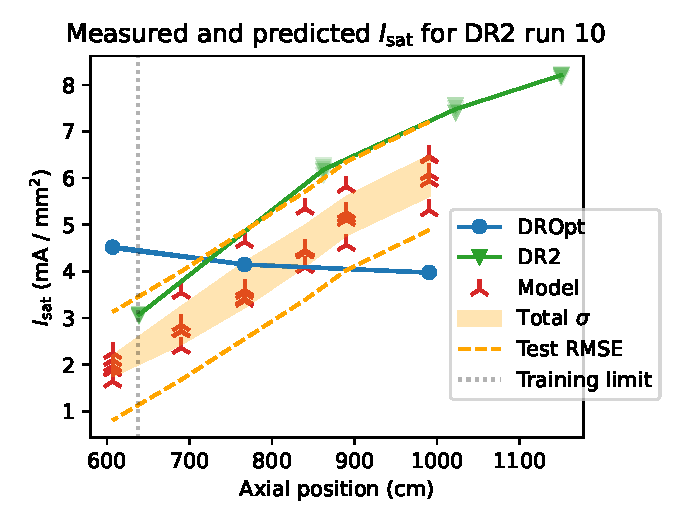
\includegraphics[width=300pt]{figures/DR2-10_LHS-30_valdiation.pdf}
	\caption[size=12]{\label{fig:DR2-10_LHS-30_valdiation}Comparison of original \texttt{DR2} profiles with the profiles from the optimization dataset (\texttt{DROpt}) for the same machine configuration. The $I_\text{sat}$ values in the \texttt{DROpt} dataset are not calibrated in this plot, indicating significant variation in probe calibration in this \texttt{DROpt} dataset.}
\end{figure}


\begin{figure}
	\centering
	\subfloat[\label{fig:DR1_vs_TS}Thomson scattering (TS) 8 ms into the discharge compared to the model predictions (10 to 20 ms averaged). Broadly speaking, the TS measurement roughly agrees with the model estimate on average. ]{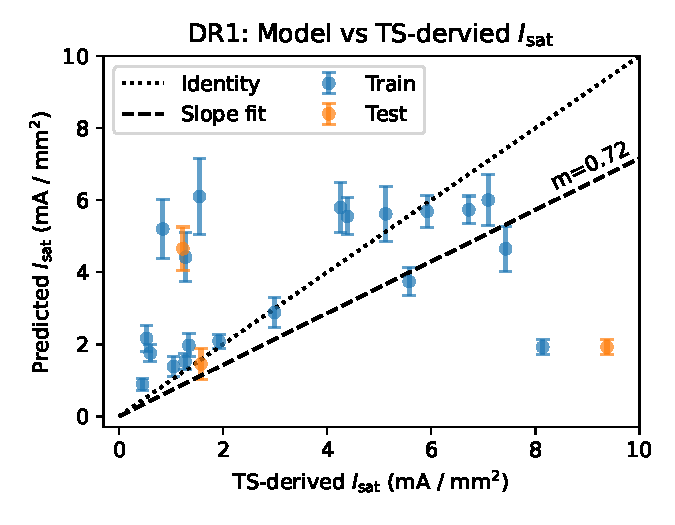
\includegraphics[width=300pt]{figures/DR1_vs_TS.pdf}}
%	\qquad
	\vfill
	\subfloat[\label{fig:DR2_vs_TS}Thomson scattering (TS) 12 ms into the discharge compared to the model predictions (10 to 20 ms averaged) and $I_\text{sat}$ measurements one port away. The TS underestimates $I_\text{sat}$ in general.]{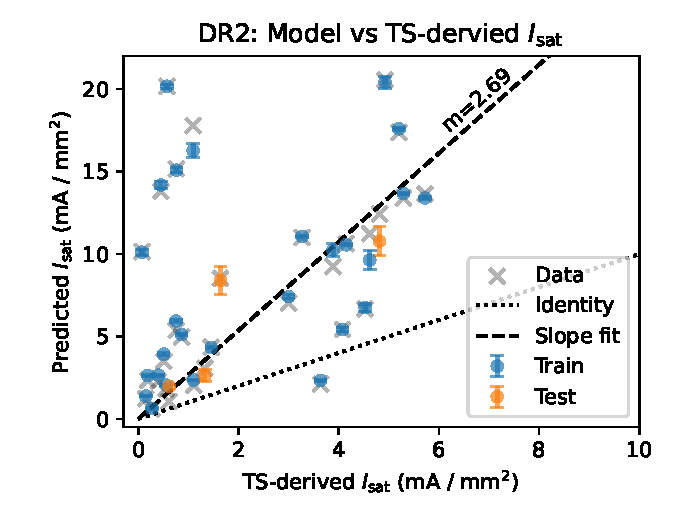
\includegraphics[width=300pt]{figures/DR2_vs_TS.pdf}}
	\caption[Comparison of $I_\text{sat}$ predictions with Thomson scattering measurements]{}
\end{figure}


\section{Inferring trends}
\label{sec:trends}

%\begin{enumerate}
%	\item Discharge voltage trends (done)
%	\item Discharge voltage trends -- real data
%	\item Axial gradient vs gas puff (done)
%\end{enumerate}

%\todo{Change this first sentence}
A systematic study of the impact of discharge voltages on $I_\text{sat}$ profiles has not been conducted using conventional techniques. Collecting both z- and x-axis profiles over a wide range of discharge voltages would take a considerable amount of time, mostly from the requirement to dismount and reattach the probes and probe drives along the length of the LAPD. This study has now been performed using the learned model, circumventing these time-consuming challenges. Model input parameters were chosen to be common, reasonable values: 1 kG flat field, 80 V gas puff, 38 ms gas puff duration, run set=\texttt{DR2}, and top gas puff off. The 38 ms puff is used in these predictions because it is the most common gas puff duration in the training set -- the model is biased in favor of this gas puff setting. The results of changing the discharge voltage only can be seen in fig \ref{fig:discharge_voltage_effect}. Notably, the $I_\text{sat}$ increases across both axes. Steeper axial gradients are seen with lower discharge voltages, but peaked x-profiles are seen at higher discharge voltages. The area closer to the source region (+z direction) appears to have a steep drop but flatter profiles down the length of the machine. 

 Unfortunately the discharge current was not included as an output in the training set. Otherwise the effect of changes in discharge power, rather than simply voltage, could be computed. The discharge current -- and thus discharge power -- is set by cathode condition, cathode heater settings, and the downstream machine configuration, and thus cannot be set to a desired value easily before the discharge. Discharge voltage, however, can remain fixed.

\begin{figure}
	\centering
	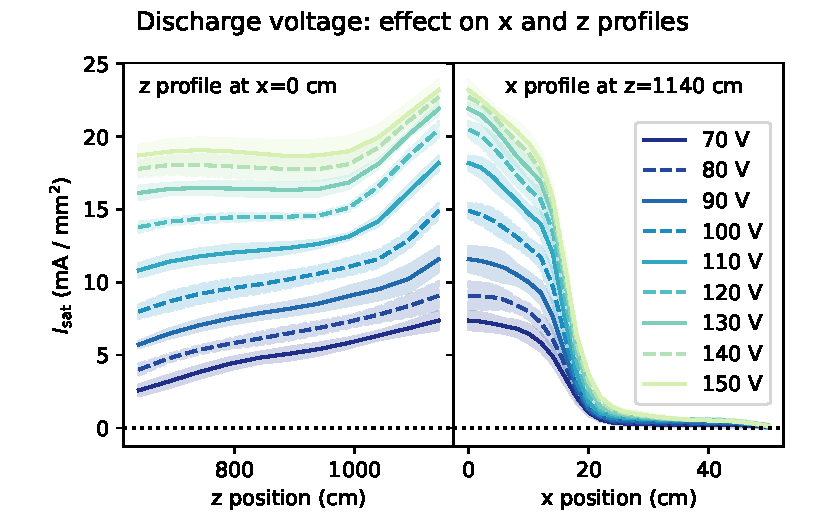
\includegraphics[width=400pt]{figures/discharge_voltage_effect.pdf}
	\caption[size=12]{\label{fig:discharge_voltage_effect}The z profile at x=0 cm and x profile at z=1140 cm for different discharge voltages. The $I_\text{sat}$ decreases with increasing voltage, and the error (filled regions) stays roughly the same, but in general increase slightly towards the cathode and at higher discharge voltages.}
\end{figure}

Of particular interest for some LAPD users is achieving the most uniform axial profile possible. We explore this problem in the context of mirrors. The gas puff duration is known to be a large actuator for controlling density and temperature and so is explored as a way of shaping the axial profile. We predict discharges with a flat 1 kG field with the probe in the center. The discharge voltage was set at 110 (a reasonable, middle value) with the run set flag=\texttt{DR2} and top gas puffing=off. The inferred effect of gas puff duration on the axial gradient and axial gradient scale length can be seen in Fig. \ref{fig:axial-grad_gas-puff.pdf}. Care was taken to handle the aleatoric (independent) uncertainty separately from the axially-dependent epistemic uncertainty. As seen in the figure, the mean axial gradient decreases when the gas puff duration is shortened. The gradient scale length also increases, so the mean gradient is not decreasing simply because the bulk $I_\text{sat}$ is decreasing. This result suggests that the gas puff duration may be a useful actuator to consider when planning future experiments. 

These applicability of these results are somewhat muted because the gas puff duration was not chosen randomly in the training discharges. 
%Only 6 runs in the training set had gas puff durations less than 38 ms. Three were 5 ms, three were 10 ms, with each having mirror ratios 1, 3, and 6 and otherwise identical configurations. The 20 ms gas puff duration datarun was in the test set. 
Given this lack of data diversity, the accuracy and applicability of this study must be interpreted cautiously. When a model is trained on \emph{all} data available (using the cross-validated test set MSE as a guide for error), which includes the 20 ms gas puff case, the predicted gradient scale length decreases uniformly across the duration scan by 1 meter. The fact that the trend remains intact when an additional, randomized intermediate gas puff case is added gives confidence in the predictions of the model despite the lack of data diversity.

\begin{figure}
	\centering
	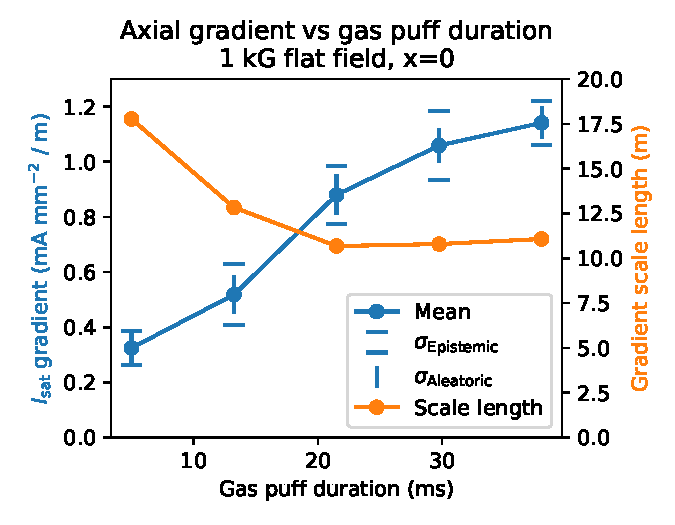
\includegraphics[width=300pt]{figures/axial-grad_gas-puff.pdf}
	\caption[size=12]{\label{fig:axial-grad_gas-puff.pdf}ML prediction: mean axial gradients decrease with decreased gas puff duration. Five durations are plotted between 5 and 38 ms (which are the bounds of the training data), evenly spaced. The gradient scale length also increases, indicating that the gradient change was not just from a decrease in the bulk $I_\text{sat}$.}
\end{figure}

\section{Optimizing profiles}
\label{sec:optimization}

%\begin{enumerate}
%	\item Table: machine settings predicted (done)
%	\item Measured vs predicted profiles (done)
%\end{enumerate}

One particular issue seen in LAPD plasmas is sharp axial density and temperature gradients. Some experiments require flat gradients, such as Alfv\'en wave propagation studies. We explore optimizing the axial $I_\text{sat}$ variation as an approximation to this problem. 
In addition, in this case the optimization problem is used as a tool to evaluate the quality of the learned model. This is a very demanding task because the trends inferred by the model along all inputs must simultaneously be accurate. Constraints on this optimization further increase the difficulty of the problem. Success in optimization provides strong evidence that the model has inferred relevant trends in predicting $I_\text{sat}$.
We quantify the uniformity of the axial profile by taking the standard deviation of $I_\text{sat}$ of 11 points along the z-axis ($x,y=0$). The required LAPD state for attaining the most uniform axial profile can be found by finding the minimum of this standard deviation with respect to the LAPD control parameters and flags:
\begin{equation}
	\text{Inputs} = \operatorname*{arg\,min}_{\text{Inputs} \neq z} \operatorname*{sd}_{z}(I_\text{sat}|_{x=0})
\end{equation}
The largest axial variation can likewise be found by finding the maximum. The model inputs used for this optimization can be found in Table \ref{tab:axial_optimization_inputs}. 

\begin{table}
	\small
	\centering
	\caption{Machine inputs and actuators for model inference}
	\label{tab:axial_optimization_inputs}
	\begin{tabular}{l l l l}
		Input or actuator & Range & Step & Count \\
		\hline
		Source field & 500 G to 2000 G & 250 G & 7 \\
		Mirror field & 250 G to 1500 G & 250 G & 6 \\
		Midplane field & 250 G to 1500 G & 250 G & 6 \\
		Gas puff voltage & 70 V to 90 V & 5 V & 5 \\
		Discharge voltage & 70 V to 150 V & 10 V & 9 \\
		Gas puff duration & 5 ms to 38 ms & 8.25 ms & 5\\
		Probe x positions & -50 cm to 50 cm & 2 cm & 51 \\
		Probe y positions & 0 cm & -- & -- \\
		Probe z positions & 640 cm to 1140 cm & 50 cm & 11 \\
		Probe angle & 0 rad & -- & --\\
		Run set flag & off and on & 1 & 2 \\
		Top gas puff flag & off and on & 1 & 2\\
		
	\end{tabular}
\end{table}

For this optimization we use an ensemble of five $\beta$-NLL-loss models with weight decay $\lambda=0$. The $\lambda=0$ model is used because it appears to give the most useful uncertainty estimate (seen in Fig. \ref{fig:extrapolation-profile-var_two}). The optimal machine actuator states are found by feeding a grid of inputs into the neural network. This variance estimate is not well-calibrated: the error of the predictions on the test set falls far outside the predicted uncertainty. However, this uncertainty can be used in a relative way: when the model is predicting far outside its training range, the predicted variance is much larger. The ranges of inputs into this model are seen in Table. \ref{tab:axial_optimization_inputs}. These inputs yield 127,234,800 different machine states (times five models) which takes 151 seconds to process on an RTX 3090 ($\approx 4.2$ million forward passes per second) when implemented in a naive way. The number of forward passes can be reduced by a factor of 51 if the x value is set to 0 cm. Note that gradient-based methods can be used for search because the network is differentiable everywhere but this network and parameter space is sufficiently small that a comprehensive search is computationally tractable.

%This minimization disproportionately penalizes outliers. 
Like any optimization method, the results may be pathologically optimal. In this scenario, the unconstrained minimal axial variation is found when the $I_\text{sat}$ is only around 1 mA/mm$^2$, which is quite small and corresponds to $1\text{-}2\times 10^{12}$ cm$^{-3}$ depending on Te. The inputs corresponding to this optimum are given in the second column of Table \ref{tab:axial_optimization_results}. This density range is below what is required or useful for many studies in the LAPD. 

Since many physics studies require higher densities, we constrain the mean axial $I_\text{sat}$ value to be greater than 7.5 mA/mm$^{2}$ (roughly $0.5\text{-}2 \times 10^{13} \text{ cm}^{-3}$). The ``run set flag'' is set to ``on'' for cases to be validated (bolded in Table \ref{tab:axial_optimization_results}) because we wish to keep the turbopumps on to represent typical LAPD operating conditions. In addition the ``top gas puff flag'' was set to `off' to minimize the complexity of operating the fueling system on followup dataruns and experiments. Turning the top gas puff valve on is predicted to decrease the average $I_\text{sat}$ by $-2$ mA/mm$^2$ for strongly varying profiles, but otherwise the shapes are very similar.
The inputs corresponding to the maximum and minimum axial variation under these constraints can be seen in columns 3 and 4 of Table \ref{tab:axial_optimization_results}. For contrast we also consider what machine settings would lead to the greatest axial variation. The results of both of these optimizations can be seen in Fig. \ref{fig:axial-var_prediction-vs-measurement}. The optimizations yield profiles that have the largest $I_\text{sat}$ values closest to the cathode, which is expected.

%As seen in Fig. \ref{fig:best_axial_var}, the predicted uncertainty and test set RMSE are very large in comparison, which indicates the model may be far outside the bounds of the training data.

The prediction for an intermediate axial variation case is also seen in Fig. \ref{fig:axial-var_prediction-vs-measurement}. The intermediate case was chosen as somewhere around half way between the strongest and weakest case with a round index number (15000, in this case). The parameters for intermediate case are also enumerated in Table \ref{tab:axial_optimization_results}. 

\begin{table*}
	\small
	\centering
	\caption{Machine inputs and actuators for optimized axial profiles}
	\label{tab:axial_optimization_results}
	\begin{tabular}{p{1.8 in} | p{0.75 in} p{0.75 in} p{0.75 in} p{0.8 in}}
		Input or actuator & Weakest & \textbf{Weakest} & \textbf{Strongest} & Intermediate \\
		$I_\text{sat}$ constraint (mA/mm$^2$) & $I_\text{sat} = $ any & $I_\text{sat}>7.5$ & $I_\text{sat}>7.5$ & $I_\text{sat}>7.5$\\
		\hline
		Source field      & 750 G   & 1000 G   & 500 G 	& 2000 G \\
		Mirror field      & 1000 G  & 750 G    & 500 G 	& 1250 G \\
		Midplane field    & 250 G   & 250 G    & 1500 G & 750 G \\
		Gas puff voltage  & 70 V    & 75 V     & 90 V 	& 90 V \\
		Discharge voltage & 130 V   & 150 V    & 150 V 	& 120 V \\
		Gas puff duration & 5 ms    & 5 ms     & 38 ms 	& 38 ms \\
		Run set flag      & on      & on       & on 	& on \\
		Top gas puff flag & on      & off      & off 	& off \\
	\end{tabular}
\end{table*}

The predicted configurations with the run set flag on and top gas puff flag off (bolded in Table \ref{tab:axial_optimization_results} were then applied on the LAPD. The data collected, compared with the predictions can be seen in Fig. \ref{fig:axial-var_prediction-vs-measurement}.

\begin{figure*}
	\centering
	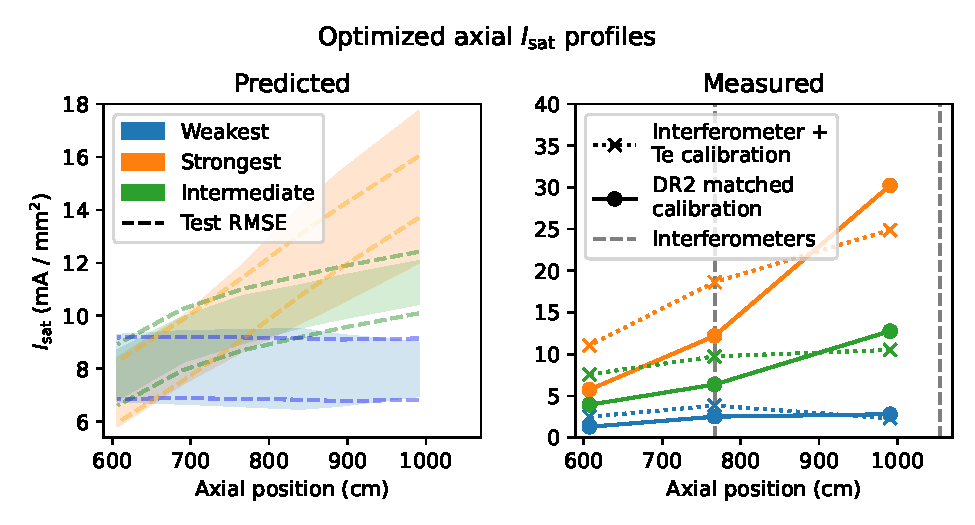
\includegraphics[width=\linewidth]{figures/axial-var_prediction-vs-measurement_paper.pdf}
	\caption[size=12]{\label{fig:axial-var_prediction-vs-measurement}Axial profiles, predicted and measured, for the optimized weakest (blue), intermediate (green), and strongest (orange) cases. a. The shaded region covers the mean prediction $\pm$ one standard deviation, and the dashed lines are $\pm$ the median cross-validation RMSE values. b. The measured $I_\text{sat}$ values are calibrated to \texttt{DR2} run 10 (solid lines), or using triple probe Te measurements on the probe and linearly extrapolating the interferometer measurements (dotted lines). The absolute values disagree between the predicted and measured values, but axial trends are consistent with the optimization.}
\end{figure*}

For the optimized axial profiles, the absolute value of the $I_\text{sat}$ predictions compared to measurement do not agree. All of the predicted profiles have overlapping predictions (within the predicted error) at the region furthest from the cathode, but the measured values do not show that behavior. Although the mean $I_\text{sat}$ value was constrained to be greater than 7.5 mA/mm$^2$, the measured mean was 2 mA/mm$^2$ for the weakest case. 

%Despite these lack  of absolute 

The important result is that the optimized LAPD settings, when implemented on the machine, do yield profiles with strong, intermediate, and weak axial variation. Although the minimum-$I_\text{sat}$ constraint was violated for the case of weakest axial variation case, this optimization would nonetheless be very useful for creating axial profiles of the desired shape. 

There are three contributing factors to the mismatch of the ML-predicted values and the real measured values. First, the condition of the machine, such as the cathode emissivity or temperature or the downstream neutral pressure, are unquantified and cannot be compensated for in data preprocessing or in the model itself. Second, the calibration of the Langmuir probes could differ substantially between runs. The probes in the training data run sets (\texttt{DR1} and \texttt{DR2}) were well-calibrated to each other within the run set, but were not absolutely calibrated. The probes used for verifying the optimization were not calibrated. A rough calibration was performed by linearly extrapolating interferometer measurements and using triple probes (dotted lines on the right panel in Fig. \ref{fig:axial-var_prediction-vs-measurement}). A configuration identical to \texttt{DR2} run 10 was also measured to simultaneously correct cathode condition and probe calibration (solid lines on the right panel in Fig. \ref{fig:axial-var_prediction-vs-measurement}). Langmuir probe calibration is discussed further in Appendix \ref{app:calib}. Third, the original dataset may not have sufficient diversity to make accurate predictions on such a constrained optimization problem.

If this optimization were performed using the dataset instead of the model, the constrained search would encompass just 10084 shots out of the 131550 shots total in the training dataset, or around 7.7\%. Including the on-axis constraint reduces the number of shots down to 303 (270 in the training set), or 0.23\% of all shots in the dataset. We conclude that this optimization of an arbitrary objective function, as done here, would be intractable using traditional, non-machine learning techniques because orders of magnitude more dataruns would need to be collected. 

Optimization requires correctly learning the trends of all inputs and how they interact. In addition, as seen from the shot statistics, the model was trained on very few shots in the constrained input and output space. These two factors -- the need for the model to learn all trends and the constrained search space -- combine to make an incredibly difficult task that functions as a benchmark for the model. These factors considered, it is not surprising that the model incorrectly predicts the absolute value. The uncertainty predicted by the model, though not well-calibrated, was nonetheless very large compared to the median test set RMSE. The model did predict the trends correctly, however; the optimized, measured profiles were strong, intermediate, or weak.

We did not check to see if the predicted optima were actually true optima: an approximation of the local derivative using a finite-difference technique would require much more run time on the LAPD than was available. 

\section{Discussion}
\label{sec:discussion}

\subsection{Key achievements}

To the authors' knowledge, this work is one of the first instances machine learning has been used to infer specific trends and optimize profiles in magnetized plasmas. Three examples of trend inference were shown in this paper: influence of magnetic geometry on plasma width, changes in the axial and radial profiles with changing discharge voltage, and the relationship of gas puff duration with axial gradient scale length. In addition, the axial profile was optimized by minimizing (or maximizing) the axial standard deviation. There is no other way of simultaneously uncovering many trends or finding optima without using an ML model trained on a diverse dataset. Traditionally, such studies would require extensive scans over grids to map the parameter space, but here it was accomplished with a relatively small amount of data.

%A few examples of trend discovery and optimization were outlined in this paper, but there are many more trends and optimizations that can be evaluated using this model.  like the one described in this paper. An optimization could be performed using a gradient-based method, Bayesian optimization, or another optimization scheme, but the process would only be applicable to one specific optimization problem.

The trends inferred in this work, such as changing discharge voltages, gas puff durations, or mirror fields, would traditionally require a grid scan (varying one parameter at a time) in LAPD settings space. Here instead we are able to extract any trend covered by the training set with only a minimal amount of machine configurations sampled. Both data collection runs lacked absolute $I_\text{sat}$ calibration and had potential differences in cathode condition. Despite these issues the model learned trends that were exploited via optimization. 

In addition, this work demonstrates uncertainty quantification broken down into epistemic and aleatoric components by using ensembles and a negative-log likelihood loss. This uncertainty estimate is useful in gauging relative certainty between different predictions of the model which increases confidence in the predictions of the model. In general, the total uncertainty predicted by the model increases when predictions are made outside the bounds of the training data. 

Fundamentally, this model can predict $I_\text{sat}$ with uncertainty at any point in space covered by the training data. No other model currently exists that can perform this prediction. Traditionally, this capability would be possible only with a detailed theoretical study. 

\subsection{Current limitations}

This study would be dramatically improved by collecting more, diverse data. Only 44 of the 67 dataruns in this dataset had randomly sampled LAPD machine settings which is very small compared to the over 60,000 possible combinations. In addition, there are many other settings or parameters that were not changed in this study, such as gas puff timings, gas puff valve asymmetries, wall/limiter biasing, cathode heater settings, operation of the north cathode, and so on. The bounds of the inputs were also conservative; all settings in this study could be pushed higher or lower with a small amount of risk to LAPD operations. In addition, the placement of the probes could be further varied and placed outside the mirror cell, which would provide a more complete picture of LAPD plasmas, particularly axial effects.

Probe calibrations differed between the two training run sets (\texttt{DR1} and \texttt{DR2}) -- and a flag was introduced to distinguish between them -- but despite this deficiency combining the two run sets was shown to be advantageous for model performance. The condition of the cathode (e.g., electron emissivity and uniformity) also has a large impact on the measured $I_\text{sat}$. The improved model performance with the flag suggests that inconsistencies between dataruns could be compensated for using latent variables if a generative modeling approach is to be taken. At the very least, this model provides a way to benchmark these differences in machine state.

Concerning the model, hyperparameter tuning could be performed. In this study a few extra percent in MSE performance is not meaningful considering the limited dataset. Instead, we focused on the trends and insights that can be extracted from this model rather than simple predictive accuracy. There may also be regimes in hyperparameter space where the uncertainty is better calibrated (perhaps using early stopping). Uncertainty estimation is important, even if the absolute uncertainty is not well-calibrated because it can provide a useful relative estimate as shown in this paper. 

Trends such as the dependence of axial gradient on the gas puff duration (fig. \ref{fig:axial-grad_gas-puff.pdf}) or the effect discharge voltage on x-z profiles (fig. \ref{fig:discharge_voltage_effect}), although intuitive, remain unverified. Verification of these trends would increase confidence of model predictions when setting LAPD parameters in future experiments.

\subsection{Future directions}

The neural network architecture used here can readily scale to additional inputs and outputs; including time-series signals is the obvious next step. Integration of multiple diagnostics -- perhaps starting with individual models before combining them -- could enable inference of plasma parameters throughout the device volume. For example, combining triple probe electron temperature measurements with existing $I_\text{sat}$ data would allow density predictions anywhere in the plasma. This capability could enable in-situ diagnostic cross-calibration (e.g., the Thomson scattering density measurement) and prediction of higher-order distribution moments like particle flux. The model could be further enhanced by incorporating physics constraints such as boundary conditions (e.g., zero $I_\text{sat}$ at the machine wall) or symmetries. 

The problem presented here -- learning time-averaged $I_\text{sat}$ trends -- is fairly simple and required a relatively simple model. As demonstrated in this work, ML provides a way to explore regions of parameter space quickly and efficiently. Most physics studies on plasma devices (and fusion devices) are dedicated to a single particular problem, use grid scans, and are not useful to other experiments or campaigns. This work shows a way of using data and trends uncovered from other experimental studies. This work also demonstrates that random exploration can be a useful tool: the increased diversity of the aggregated data will generally benefit an ML model whether the experimenter discovers something new or not.

\section{Conclusion}
\label{sec:conclusion}

We demonstrate the first randomized experiments in a magnetized plasma experiment to train a neural network model. This learned model was then used to infer trends when changing field configuration, discharge voltage, or gas puff duration. This model was also used to optimize axial variation of $I_\text{sat}$ as measured by the standard deviation, which was validated in later experiments despite poor absolute error. 

We strongly advocate that all ML-based analyses in plasma and fusion research should be validated  and used to gain insight by inferring trends, as demonstrated here. This validation step is crucial for ensuring that ML models capture physically meaningful relationships and the insights provided may provide direction for future research. We hope this is the first step towards automating plasma science.
%\pagebreak


%\section{Acknowledgements}

%The authors would like to thank Prof. Walter Gekelman, Prof. Christoph Niemann, Dr. Shreekrishna Tripathi, Dr. Steve Vincena, Dr. Pat Pribyl, Tom Look, Yhoshua Wug, Dr. Lukas Rovige, and Dr. Jia Han for insightful discussions and experimental support.

%\setcounter{section}{1} % reset numbering

\section{The open dataset and repository} 
\label{app:repo}
All the code to perform the ML portion of this study is available at \url{https://doi.org/10.5281/zenodo.15007853}. The training datasets are also available in that repository in the \texttt{datasets} directory. Additional data are available upon request. The repository also contains additional training details and the notebooks for generating the plots in this document. 
The plots used in this paper were made in jupyter notebooks, which are also uploaded. The final training code can be found in \texttt{train\_dense\_beta\_NLL.py}. Trained models are found in the \texttt{code/training\_runs} directory.
The history of many training runs can be found on Weights and Biases: \url{https://wandb.ai/phil/profile-predict} and the accompanying notes on these trained models are found in the associated pdf on github.
The code and dataset are licensed under Creative Commons Attribution Share Alike 4.0 International. 
